\documentclass{article}
\usepackage[english]{babel}
\usepackage{url}
\usepackage{graphicx}
\usepackage{amsthm}
\usepackage{hyperref}
\usepackage[round, authoryear, super]{natbib}
\bibliographystyle{chicago}

\begin{document}
	\begin{titlepage} 
		\centering
		{\scshape\Large Dikult 105\par}
		\vspace{2em}
		{\scshape\large Candidate Number: 137\par}
		\vspace{6em}
		{\scshape\Large Assignment number?\par}
		{\scshape\LARGE A clash of colours.\par}
		\vspace{1em}
		{\scshape\url{http://designconference.aiga.org/#!/}\par}
		\vfill
		{\scshape Word count: 0000\par}
		\vspace{3em}
		\large\today
	\end{titlepage}

	\begin{figure}[h!]
        \centering
        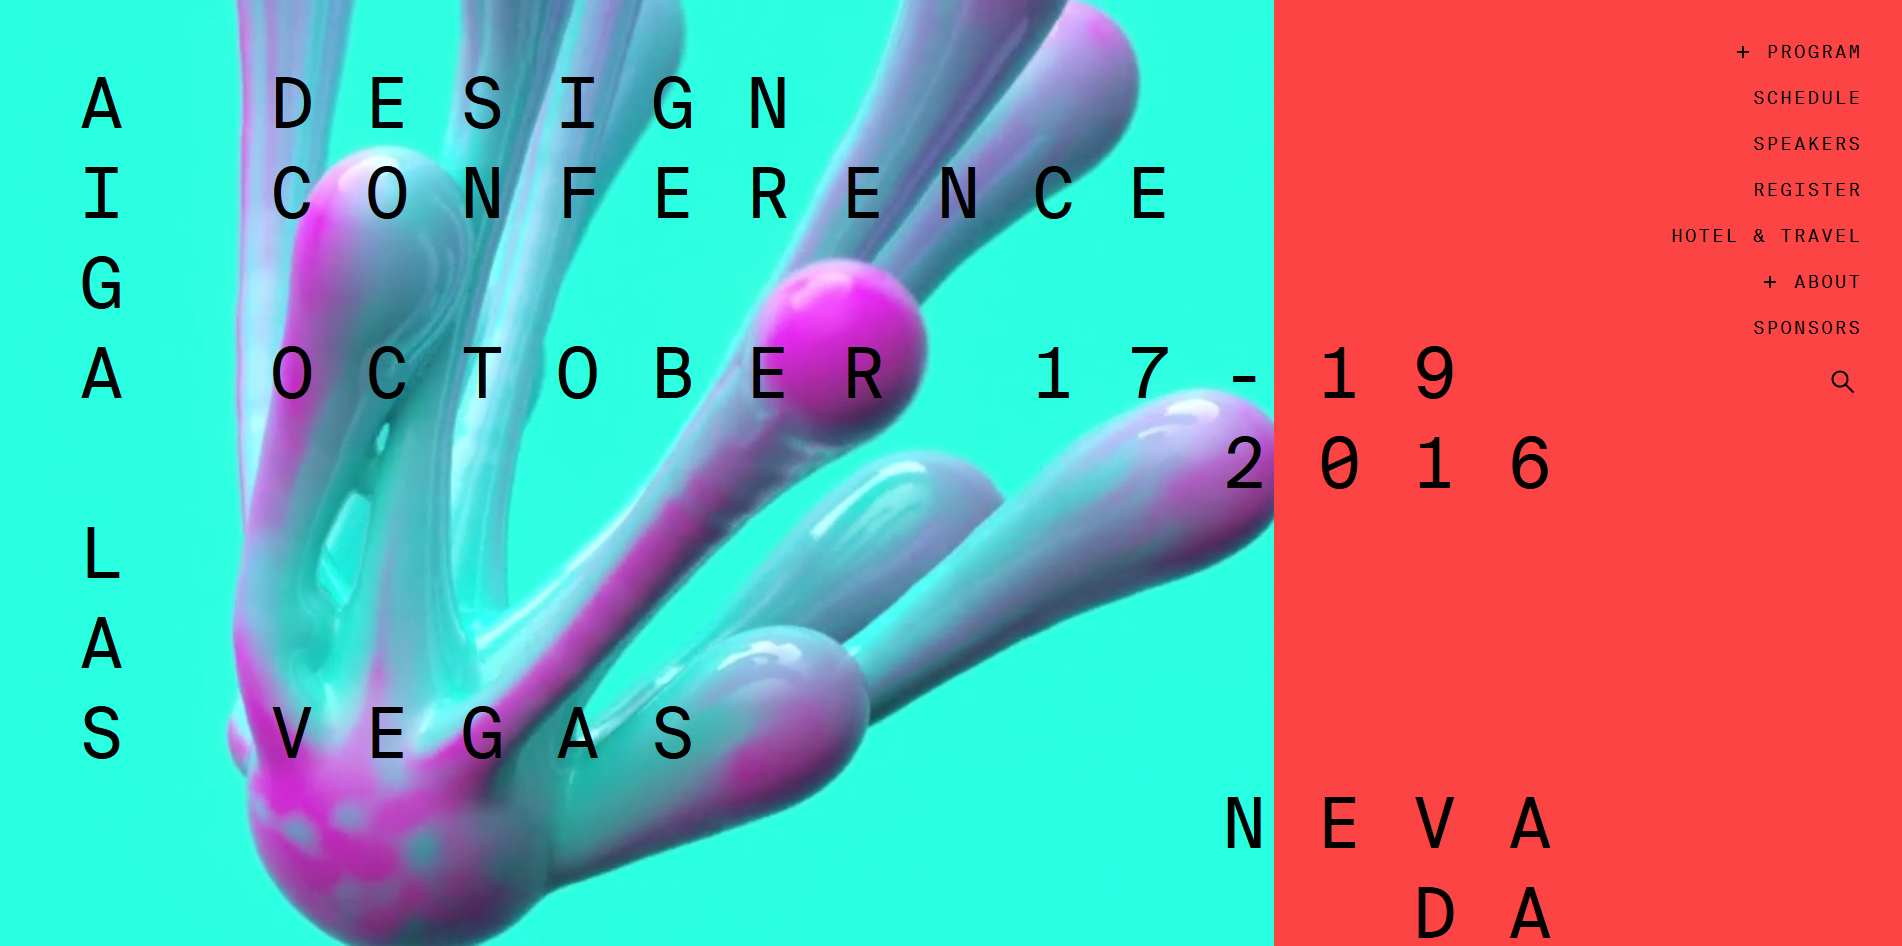
\includegraphics[width=0.8\textwidth]{frontPage}
        \caption{The front page of the website http://designconference.aiga.org/}
    \end{figure}
    \vspace{5em}
	\section{Preface}
	    Balanced, and yet not. Controlled, but flawed. Sleek, and stressful. These are some of my first impressions when entering this website. Steve Jobs said in an interview while talking about design that: "It's not just what it looks like and feels like. Design is how it works."\citep*{SteveJobsQuote} And I agree, but it is important how it looks and feels; and while i was initially sceptical and a bit taken aback by this. However the analytical process gave me time to dwell on much of the initial scepticism. This will be explain more in the design-section of the analysis. Working my way through this sites navigational elements I will show how they can be seen as a metaphor for Las Vegas and the atmosphere the city and indeed the name gives.
    \section{Introduction}
	    The AIGA (The American Institute of Graphic Arts) conference website is part of the awwwards collection of websites using unusual navigation. Aiga is a community of design advocates and practitioners where members can learn, help, share and create content that makes the design community thrive. The website I have chosen is for the yearly conference that AIGA hosts, where members can go to and listen to selected speakers and gather as a community. The AIGA conference that was hosted this year in October was a milestone for the Institute. Therefore this website was clearly made for drawing members of AIGA to the conference and give them the information they need/want to have. I chose this site then because the way it cached my eye and the chance of analysing a website made by designers, for designers. 
    \section{The analysis}
	    \subsection{The squid in the room -focal points, shapes and colours}
		    There are many things to discuss and analyse about this website and the first object on the agenda is the huge abstract figure flowing down the screen. "A focal point is any element on a page that draws the viewer’s eye" \citep[Page. 22]{PWebDesign}. The figure here is working well as a metaphor for the ever changing community of design and the fluidness of what is defined as design. And more working as a focal point, that is exiting enough to make a user stay on the website rather than discard it like so many other websites. \\More than giving the front page something to look at, the figure in the background might represent the floating and evolving of web design as a whole. As Beaird says in his book - "Freeform shapes have a free-flowing nature that conveys a sense of informality and spontaneity"\citep[Page. 86]{PWebDesign} So it is more than giving a focal point the figure in the background.\\ The shape conveys that the website is informal and spontaneous and navigates you downwards with its motion. This urges you to scroll down and get more information, giving more to the idea of evolving from the simple letters and figures at the top to a more complex world below. The free-form shape in the background also offsets the strict and rectangular feel that the rest of the website creates and gives the user a sense of a more organic and smooth website. All the boxed further down the page is completely fixed and solid so the fluency the shape gives really compliments the rest of the page. \\This also complements the way the text is structure. Just like the figure the text comes in gradually and announces itself. This gives the letters importance and since this is a conference it fits nicely to the theme. Giving it the structure the text has gives meaning with the different proximity of the letters. Here the words gives their own focal point and gives the feeling of reading words rather than just scattered letters.\\
            The symbolic of colours are also very important and giving the shape the colours that they have done reflects their knowledge of colour psychology. The cold turquoise colour mixed with the warmer pink provides the front page a lot of depth on an emotional level too. The cool turquoise are calming and the pink gives a hint of heat and motion, much like the shape itself. \citep[Page. 50]{PWebDesign} 
        \subsection{The inefficient wall -Design structure}
        Balance, structure and the rule of thirds. These are some of the concepts that are important for giving importance for the content, to guide where the user should look and what the user should feel.
        \begin{figure}[!h]
            \centering
            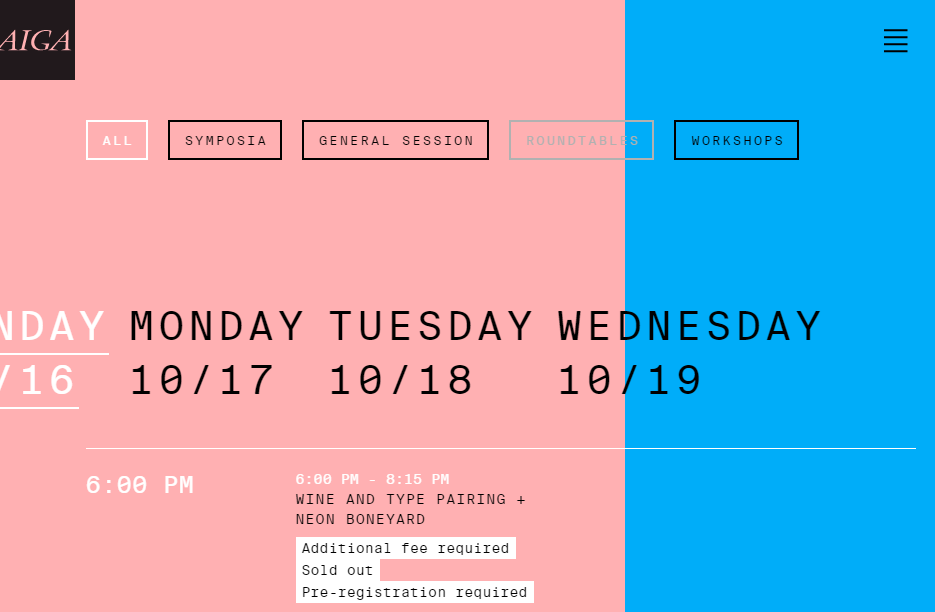
\includegraphics[width=0.8\textwidth]{LineBreaker}
            \caption{An example from the schedule section of the site where the vertical line breaks the page into two sections. }
        \end{figure}
        As seen in figure 2 the vertical line going down splits the page into two parts; content origin and main navigational. This creates a barrier that the content origin side breaks constantly and violates, creating drama and excitement on the page. "The rule of thirds says that dividing a layout or composition into thirds makes for a more interesting visual composition." - \cite[Page. 252]{WSINYE}. By constantly breaking this line and deepening the layers of each page. These pages gain something that is very difficult to put a finger on and although seeming like counter-intentional creating a more stress-like environment, it works very well as a symbol for the stress and the hectic world of Las Vegas.\\ The vertical lines effect is also amplified by the subtle effect of having a heavier and more defined colour on the right side. Giving the effect of lightness and ease for the content with its light and diffuse colour. This is not just the case for the example in figure two, but the site consistently puts a heavy colour on the right and a lighter on the left. The light area gives a subtle, floating feeling to the page that is being observed and hints that there are more dimensions to the page. What this allows is to compliment the other side of the line, more depth. Gaining this the navigational area seems heavier and symbolizes to the user that the are is solid and that it can be trusted. Used for when there is something the user needs. It is important to note that the weight does not really draw draw the eye away from the content, but rather ensures it thanks to the use of the rule of thirds.\\  
        \subsection{The multi dimensional navigational elements -Navigation}
        As established the weight of the right side gives ground for a navigation system. A simple hamburger icon at the top right of the page. So a simple menu icon for a complicated page. More so when the user have navigated away from the front page to pages where there are more and noisier content. The way this refuses the user the possibility to just glance at the menu can be a metaphor for the casinos in Las Vegas without clocks and windows. Making you forget the time and this is re-enforced by reminding the users that the event takes place in Las Vegas throughout the content.
        \begin{figure}[!h]
            \centering
            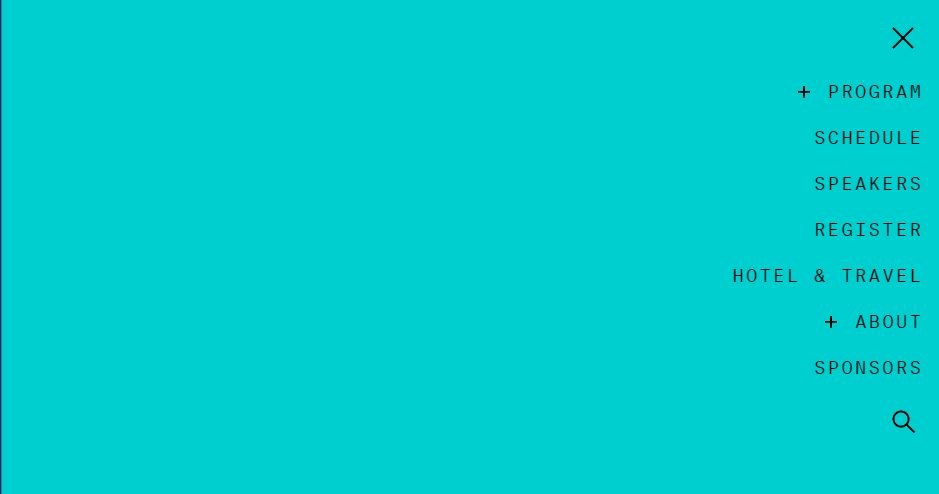
\includegraphics[width=0.8\textwidth]{NavMenu}
            \caption{The hamburger icons transformation of the page to the navigational area.}
        \end{figure}
        When clicking the hamburger menu this is when the websites structure gets redefined. Casting aside the rule of thirds and not changing colour gives a steady and familiar feeling where there should be. Not having to adapt to a new complex page and just finding this simple screen when the navigational element can be confusing gives a good overview and safety. Here the turquoise colour again gives a feeling of calm and that is what the user needs. Other than the points above this element is just an expandable list of items and sub-items where navigation goes quite smoothly and is relatively fast.\\
        More than this simple overlaying navigation system, many of the pages has a wide range of internal-sub-navigational elements and/or filtering, giving a deeper feeling to the page. This can be observed in figure 2 where the current page is the 
    \section{Conclusion}
    Having thought trough the design choices and reconsidered my first impressions I have to conclude that not only does this site present the information to the users in an exiting and functional way, but it actually seems to be quite balanced and the more time I spent on the site the less i felt those initial prejudices I had upon entering the website. I have seen that the vertical line and   completely shattered my 
    \bibliography{BookReferences}
    
    
        
    
\end{document}

